\section*{Introduccion}
\addcontentsline{toc}{section}{Introduccion}
%Small description \cite{lehman2006biblatex} 
%en la figura \ref{figura1} tabla \ref{tabla1}
Linux es el sistema operativo mas usado del mundo, aprender a usarlo puede ser algo intimidante la inicio pero con el tiempo no te querrás despegar de este sistema, su estabilidad y constante actualización hace de linux uno de los sistemas mas seguros y personalizables, es el sistema favorito por los hackers desarrolladores y entusiastas del software libre.
\\
Soy usuario activo de linux desde el 2012 aunque la primera vez que lo probé fue por el
2011, use muchas distribuciones Backtrack, Linux Mint, Ubuntu, Debian y finalmente me
quede usando Debian
\section*{Requisitos}
Para poder hacer los ejercicios de esta guia necesitaras un sistema linux, ya sea
maquina fisica, virtual o tambien el kernel de linux disponible en windows.
\section*{Posibles usos de linux}
\begin{enumerate}
  \item Edicion de video o música, aunque la gran mayoria de programas estan en windows, linux cuenta con algunos programas muy potentes como por ejemplo
    \begin{enumerate}
      \item Davinci Resolve(Edición de Video profesional)
      \item Kdenlive(Edición de Video, completo y de bajos requisitos)
      \item Reaper(Edición de audio)
      \item Audacity(Edición de audio)
    \end{enumerate}
  \item Video juegos, aunque no es el mejor tenemos algunas soluciones
\begin{enumerate}
  \item Wine, para emular un sistema windows y poder correr algunos juegos, aunque
no es algo 100 \% seguro
\item Lutris, usa wine por debajo y también puede correr juegos emulando un sis-
tema windows, este lo he probado y logre jugar World of Warcraft, Starcraft
Remastered, Starcraft 2
\item Steam, de soporte para linux 100\% en sus juegos como Dota2, CS2, etc. En
steam hay gran cantidad de juegos y estos pueden ser instalados siempre y
cuando cuenten, steam tambien cuenta con proton que nos permite instalar juegos de windows.
\end{enumerate}
  \item Desarrollo de software, aquí es el Dios indiscutible, aunque apple usa unix linux sigue siendo la preferida por el control que el usuario siente al usarla.
  \item Oficina, LibreOfice es la opción pero ten cuidado de guardar los archivos en el formato correcto.
\end{enumerate}
\section*{Mascota de Linux TUX}
Mascota oficial de linux
\begin{center}

\includegraphics[width=0.5\textwidth]{image/chapter_01/tux.png}
\end{center}

\begin{lstlisting}[language=python,caption={Python example}]
def test(name):
	print(name)
\end{lstlisting}

%\begin{table}[h]
%	\centering
%	\begin{tabular}{l | l | l}
%		A & B & C \\
%		\hline
%		1 & 2 & 3 \\
%		4 & 5 & 6
%	\end{tabular}
%	\caption{very basic table
%	\label{tab:abc}
%\end{table}

\begin{table}[h]
	\centering
	\begin{tabular}{| l c r |}
		\hline
		1 & 2 & 3 \\
		4 & 5 & 6 \\
		7 & 8 & 9 \\
		\hline
	\end{tabular}
	\caption{A simple table}
	\label{tabla1}
\end{table}

\begin{figure}[h]
	\centering
	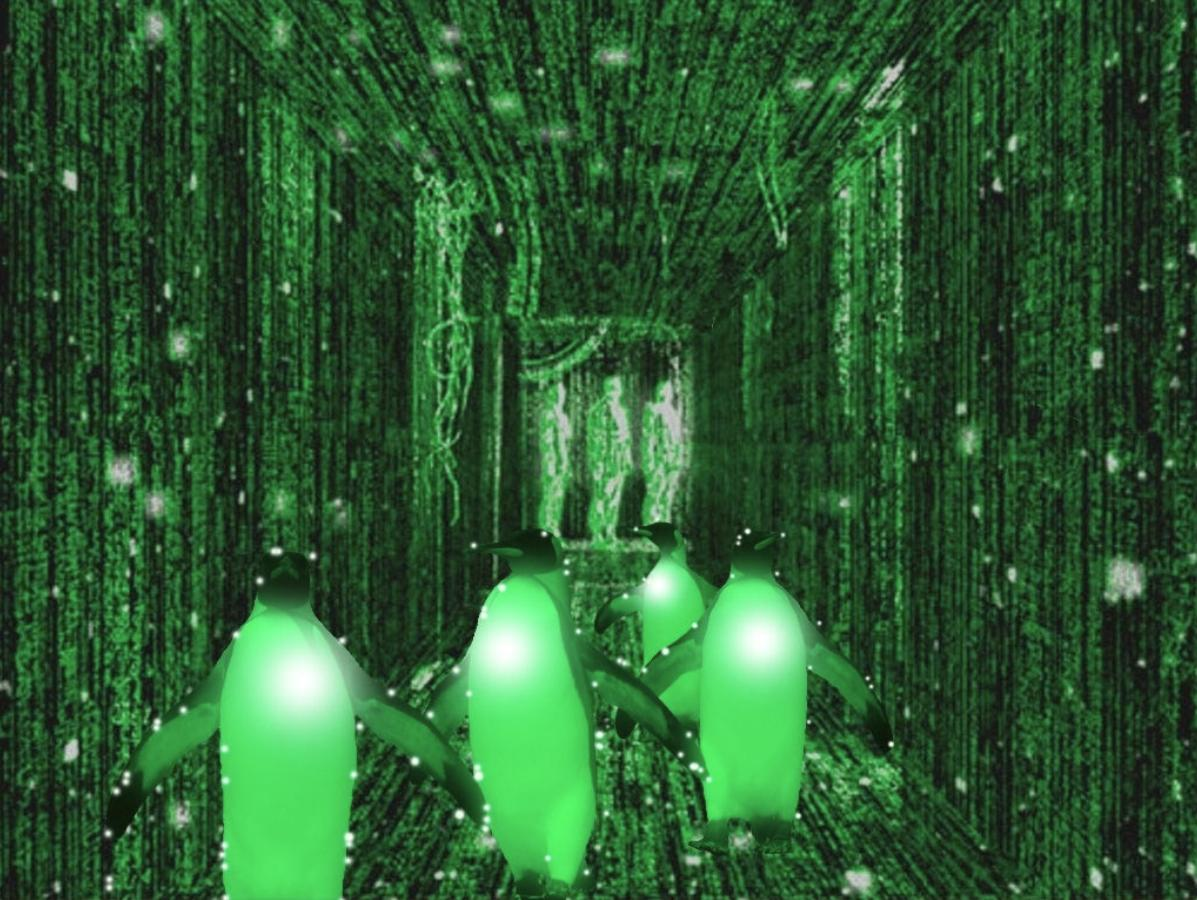
\includegraphics[width=0.5\textwidth]{image/cover.jpg}
	\caption{Figure description.}
	\label{figura1}
\end{figure}
